%%%%%%%%%%%%%%%%%%%%%%%%%%%%%%%%%%%%%%%%%%%%%%%
\chapter{Network Coding} \label{chap:network_coding}
%%%%%%%%%%%%%%%%%%%%%%%%%%%%%%%%%%%%%%%%%%%%%%%

\section{What is Network Coding?}

The most general definition of Network Coding is defined in the seminal
paper of Ahlswede \textit{et al.} \cite{Ahlswede:2000}. It refers
to \textit{coding} at a vertex in a network, where coding means an
arbitrary combination of inputs for outputs. This combination is called
a \textit{network code}. Because this coding process does not only
happen at the source but on any vertex in the network, the network
codes are on \textit{packets}. Packets can be messages of the sources
or inputs of a vertex. Ahlswede \textit{et al.} look at networks consisting
of vertices interconnected by error-free point-to-point links, which
is still applicable to present-day networks, e.g. error-free wireline
networks. The study of ``error-free links'' in network coding distinguish
itself from Channel Coding for noisy links.

A particular form of network coding is \textit{Random Linear Network
Coding} - RLNC introduced in \cite{Ho:2003}. RLNC considers each
vertex's outputs as a linear combination of its inputs, specified
by independent and randomly chosen code coefficients from some finite
field $\ensuremath{\mathbb{F}}_{q}$. These coefficients can be represented
in a vector as extra information for an initial packets, which is
able to be contained in packet headers of the present-day widely used
network called \textit{Packet Network}. Hence, in this study, we define
\textit{Network Coding} as coding at a vertex in a packet network,
where data are divided into packets and network code is applied to
the contents of packets. This concept is clearly explained in Section
\ref{subsec:Scalar-network-coding}, Section \ref{subsec:Vector-network-coding},
and Section \ref{subsec:Matrix-channel}, where we introduce scalar
and vector network coding as a matrix channel.

\section{Advantages of Network Coding}

\subsection{Throughput gain and reduced complexity}

Network coding gives a potential gain in throughput by communicating
more information with fewer packet transmissions compared to the routing
method. The butterfly network in \cite{Ahlswede:2000} as a multicast
in a wireline network is a standard example for an increase of throughput. 

\begin{figure}[H]
\caption{The butterfly network \label{fig:The-butterfly-network}}

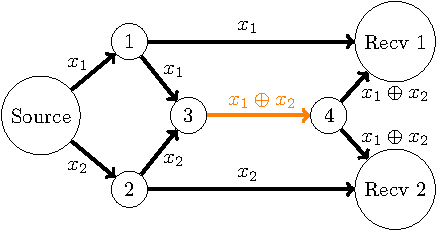
\includegraphics[width=0.5\paperwidth]{E:/Documents/TUM/THESIS/thesisCOD_Ha/figures/ahlswede_butterfly_network}
\end{figure}

In Figure \ref{fig:The-butterfly-network}, we denoted a receiver
by ``Recv'', which is used for all of figures in this study. With
help of network coding, both reveiver 1 and 2 can recover $x_{1}$
and $x_{2}$ by a bitwise XOR. Without network coding, an additional
transmission between vertex 3 and 4 must be supplemented to communicate
the contents of 2 packets $x_{1}$ and $x_{2}$ from the source to
Recv 1 and Recv 2, i.e. we must communicate $x_{1}$ or $x_{2}$ separately
on this link twice under routing. 

\subsection{Robustness}

\textit{Packet loss} is a particular issue in wireless packet networks
due to several reasons, e.g. buffer overflow or communication failures.
Sharing a common concept with Erasure Coding (EC) by exploiting a
degree of redundancy to packets on any vertices in the network, the
receivers are able to successfully recover the original packets from
a large number of packet losses, e.g. $101\circledast10\circledast1$.
The only difference is that packets are only encoded by the source
in EC \cite{Fujimura:2008}. This problem is dealed by acknowledgement
messages in the mechanism of transmission control protocol (TCP).

\subsection{Security}

Network coding offers both benefits and drawbacks regarding to security.
For example, node 4 is operated by an eavesdropper and it obtains
only the packet $x_{1}\oplus x_{2}$, so it cannot obtain either $x_{1}$
or $x_{2}$ and the communication is secure. Alternatively, if the
eavesdropper controls node 3, it can anonymously send a fake packet
masquerading as $x_{1}\oplus x_{2}$, which is difficult to detect
in network coding \cite{Ho:2008}.

\subsection{Increase the number of possible vertices}

Data in the digital communication of today are represented in binary
field, i.e. $\ensuremath{\mathbb{F}}_{2}$, so the coding coefficients
are binary numbers. When we accomodate them into packets over $\ensuremath{\mathbb{F}}_{2}^{t}$
with $t\geq2$, it has been studied in \cite{Ebrahimi:2011,Wachter-Zeh:2018}
showing that the so called vector network coding provides more possible
vertices or more connected devices in a network compared to the linear
network coding. In other words, network coding provides high adaptability
for the worldwide network's requirement by extending the base field
of packets. 

\section{Network Model}

The ``packet network'' is practical, but difficult to accurately
modelled. Hence, we introduce in next section the generalized combination
network, where supports in varying a number of \textit{connections},
specifically multicast (1 source to multiple receivers). Transmission
rate is not regulated, so we do not consider congestion control in
our network type \cite{Ho:2008}.

\clearpage